\documentclass[12pt,a4paper]{article}

\usepackage[margin=1in]{geometry}
\usepackage{graphicx}
\usepackage{float}
\usepackage{amsmath}
\usepackage{booktabs}
\usepackage{parskip}
\usepackage{hyperref}
\hypersetup{colorlinks=true, linkcolor=blue, urlcolor=blue}

\title{
    \Large \textbf{Electronic Devices \& Circuits Laboratory} \\[0.5em]
    \LARGE \textbf{Experiment 1} \\[0.3em]
    \large V--I Characteristics of PN Junction \& Zener Diodes,\\
    Clipper and Clamper Circuits
}
\author{Bhargav K \quad (EE25BTECH11013) \\ Department of Electrical Engineering \\ IIT Hyderabad}
\date{}

\begin{document}
\maketitle
\tableofcontents
\newpage

\section{Aim}
\begin{itemize}
    \item To plot the forward and reverse V--I characteristics of a PN junction diode and find its cut-in voltage, static and dynamic resistance, and reverse saturation current.
    \item To plot the forward and reverse V--I characteristics of a Zener diode and find its breakdown voltage $V_Z$ and Zener resistance $R_Z$.
    \item To design and test positive, negative and biased clipper circuits, and positive and negative clamper circuits, and record the input-output waveforms.
\end{itemize}

\section{Components Used}
\begin{table}[H]
\centering
\begin{tabular}{lll}
\toprule
\textbf{Component} & \textbf{Value/Part} & \textbf{Qty} \\
\midrule
PN junction diode & 1N4007 / 1N4148 & 1 \\
Zener diode & 1N4733A ($V_Z = 5.1$ V) & 1 \\
Regulated DC supply & 0--30 V & 1 \\
Function generator & 0--1 MHz & 1 \\
CRO / DSO & 20 MHz & 1 \\
Digital multimeter & -- & 2 \\
Resistors & 1 k$\Omega$, 4.7 k$\Omega$, 10 k$\Omega$ & as needed \\
Capacitor & 0.1 $\mu$F & 1 \\
Breadboard, wires, probes & -- & as needed \\
\bottomrule
\end{tabular}
\end{table}

\section{PN Junction Diode}

\subsection{Theory}
A PN junction diode conducts mainly in one direction. In forward bias, once the applied voltage crosses the cut-in voltage $V_\gamma$ (about 0.7 V for silicon), the current starts rising very fast for a small increase in voltage, because majority carriers are being injected across the junction in large numbers. In reverse bias, only a small reverse saturation current $I_0$ flows due to minority carriers, and this stays almost constant until breakdown happens at a large negative voltage.

The diode current is approximately given by the diode equation:
\begin{equation}
    I = I_0 \left( e^{V/\eta V_T} - 1 \right)
\end{equation}
where $V_T$ is the thermal voltage ($\approx 26$ mV at room temperature) and $\eta$ is the ideality factor.

From the forward characteristic we can find:
\begin{itemize}
    \item \textbf{Static resistance} at a point: $R_{DC} = V/I$
    \item \textbf{Dynamic resistance} near a point: $R_{AC} = \Delta V/\Delta I$
\end{itemize}

\subsection{Circuit and Simulation (Forward Bias)}
The circuit was simulated in LTSpice with a 1 k$\Omega$ series resistor and the supply swept from 0 to 0.5 V in steps of 0.1 V, followed by finer steps near the knee.

\begin{figure}[H]
    \centering
    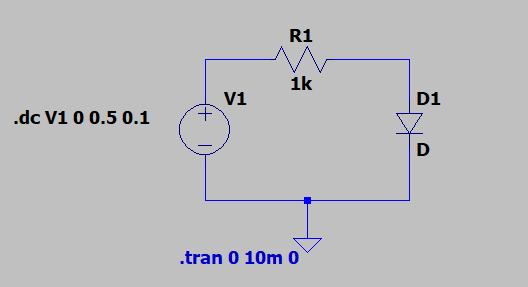
\includegraphics[width=0.6\textwidth]{E1/pnjunction/ckt.png}
    \caption{LTSpice circuit for PN junction diode forward bias test}
\end{figure}

\begin{figure}[H]
    \centering
    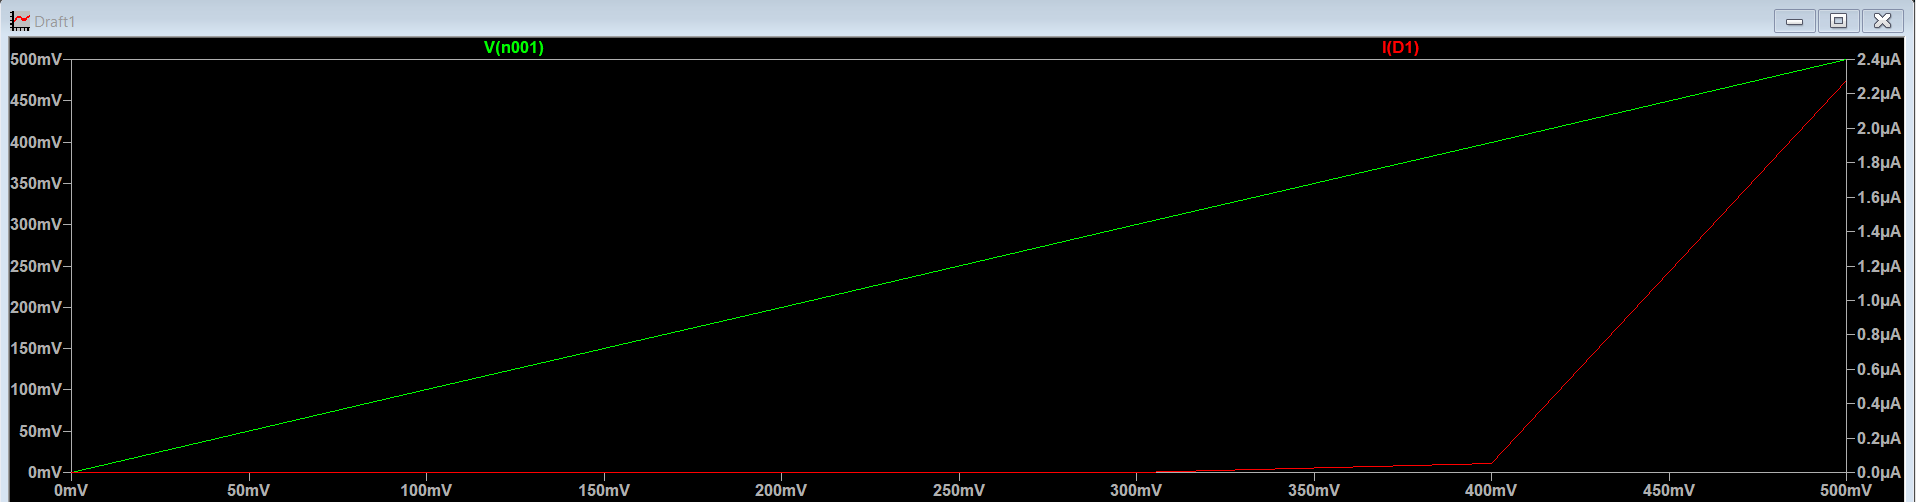
\includegraphics[width=0.85\textwidth]{E1/pnjunction/sim1.png}
    \caption{Simulated V--I plot: voltage across diode (green) and diode current (red) vs. sweep voltage. Current stays near zero till about 0.4 V and then rises sharply, showing the cut-in behaviour.}
\end{figure}

\begin{figure}[H]
    \centering
    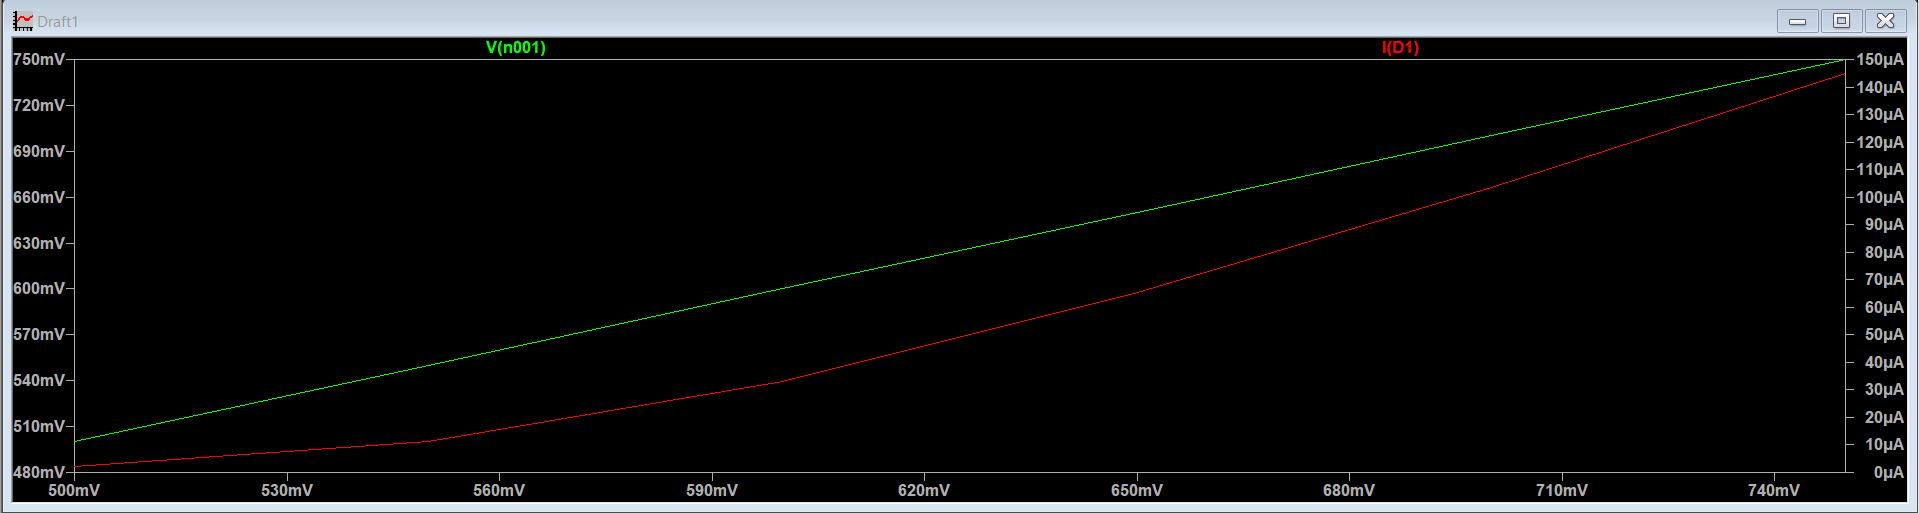
\includegraphics[width=0.85\textwidth]{E1/pnjunction/sim2.png}
    \caption{Simulated forward V--I characteristic, second view}
\end{figure}

\begin{figure}[H]
    \centering
    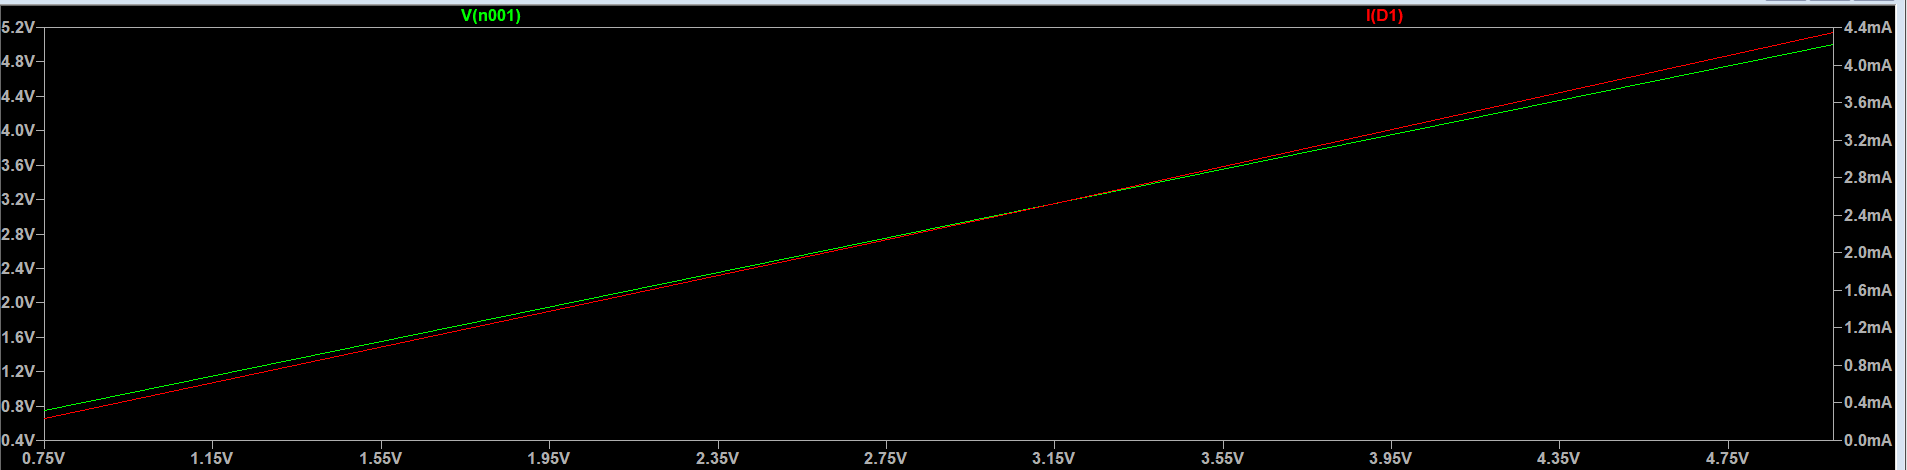
\includegraphics[width=0.85\textwidth]{E1/pnjunction/sim3.png}
    \caption{Simulated forward V--I characteristic, third view}
\end{figure}

From the simulation, the cut-in voltage is close to 0.4--0.5 V for the SPICE model used (this will be verified against the measured value from the actual diode in lab, which is usually closer to 0.6--0.7 V for silicon).

\subsection{Observation Table -- Forward Bias (to be filled in lab)}
\begin{table}[H]
\centering
\begin{tabular}{ccc}
\toprule
S.No. & $V_f$ (V) & $I_f$ (mA) \\
\midrule
1 & & \\ 2 & & \\ 3 & & \\ 4 & & \\ 5 & & \\ 6 & & \\ 7 & & \\ 8 & & \\
\bottomrule
\end{tabular}
\end{table}

\subsection{Observation Table -- Reverse Bias (to be filled in lab)}
No simulation was done for this part since the reverse saturation current of a real diode model is very small and not reliably captured in LTSpice's default diode model. This will be measured directly in the lab using a microammeter.
\begin{table}[H]
\centering
\begin{tabular}{ccc}
\toprule
S.No. & $V_r$ (V) & $I_r$ ($\mu$A) \\
\midrule
1 & & \\ 2 & & \\ 3 & & \\ 4 & & \\ 5 & & \\ 6 & & \\ 7 & & \\ 8 & & \\
\bottomrule
\end{tabular}
\end{table}

\section{Zener Diode}

\subsection{Theory}
A Zener diode is a heavily doped PN junction meant to be operated in reverse breakdown without getting damaged. Its forward characteristic is the same as a normal diode. In reverse bias, once the voltage reaches the Zener voltage $V_Z$, the current increases sharply while the voltage stays almost constant -- this near-vertical knee is what makes it useful as a voltage reference. Breakdown below about 5 V is mainly due to the Zener effect (field emission), and above about 6 V it is mainly avalanche multiplication.

The Zener resistance is calculated from the slope of the breakdown region:
\begin{equation}
    R_Z = \frac{\Delta V_Z}{\Delta I_Z}
\end{equation}

\subsection{Observations}
This part was not simulated -- it will be done directly in the lab with the 1N4733A Zener diode, since the exact breakdown behaviour depends on the physical device and is best measured directly rather than simulated.

\begin{table}[H]
\centering
\begin{tabular}{cccc}
\toprule
S.No. & $V_f$ (V) & $I_f$ (mA) & $V_r$ (V) / $I_r$ (mA) \\
\midrule
1 & & & \\ 2 & & & \\ 3 & & & \\ 4 & & & \\ 5 & & & \\ 6 & & & \\ 7 & & & \\ 8 & & & \\
\bottomrule
\end{tabular}
\end{table}

From the reverse plot, $V_Z$ and $R_Z$ will be read off from the near-vertical breakdown knee.

\section{Clipper Circuits}

\subsection{Theory}
A clipper circuit cuts off part of a waveform above or below some reference level using a diode. Series clippers pass the signal only when the diode conducts; shunt clippers use the diode to short the unwanted part of the signal to a reference level. Clippers are useful for waveform shaping and for protecting circuits from over-voltage.

\subsection{Positive Clipper (clips above +1 V)}
Here the diode conducts and clamps the output to +1 V whenever the input goes above +1 V. Below that, the diode is off and the output follows the input.

\begin{figure}[H]
    \centering
    \includegraphics[width=0.55\textwidth]{{E1/clipper/Positive clipper/ckt}.png}
    \caption{Positive clipper circuit -- LTSpice}
\end{figure}

\begin{figure}[H]
    \centering
    \includegraphics[width=0.85\textwidth]{{E1/clipper/Positive clipper/sim}.png}
    \caption{Positive clipper: input and output waveforms}
\end{figure}

The expected clipping level is:
\begin{equation}
    V_{out,max} \approx V_{ref} + V_\gamma
\end{equation}

\subsection{Negative Clipper (clips below -1 V)}
This is the mirror case of the positive clipper -- the diode is reversed so the output is clamped whenever the input goes below $-1$ V.

\begin{figure}[H]
    \centering
    \includegraphics[width=0.55\textwidth]{{E1/clipper/Negative clipper/ckt}.png}
    \caption{Negative clipper circuit -- LTSpice}
\end{figure}

\begin{figure}[H]
    \centering
    \includegraphics[width=0.85\textwidth]{{E1/clipper/Negative clipper/sim}.png}
    \caption{Negative clipper: input and output waveforms}
\end{figure}

\subsection{Biased (Two-Level) Clipper}
This combines both circuits above at the same output node -- one diode referenced to +1 V clips the top of the waveform and the other referenced to $-1$ V clips the bottom, giving a doubly clipped output.

\begin{figure}[H]
    \centering
    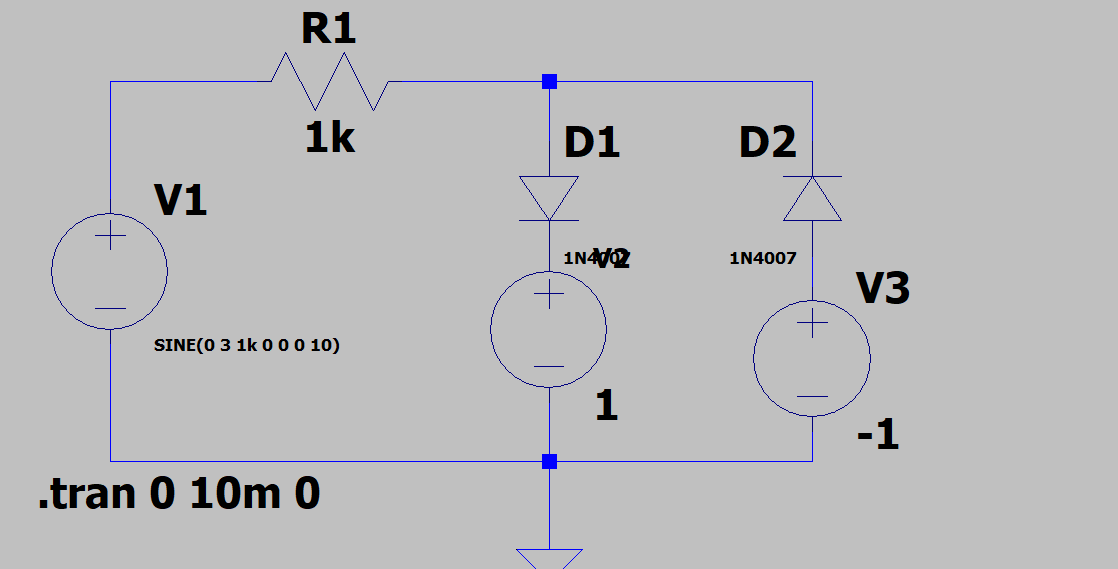
\includegraphics[width=0.55\textwidth]{E1/clipper/Biased/ckt.png}
    \caption{Biased clipper circuit -- LTSpice}
\end{figure}

\begin{figure}[H]
    \centering
    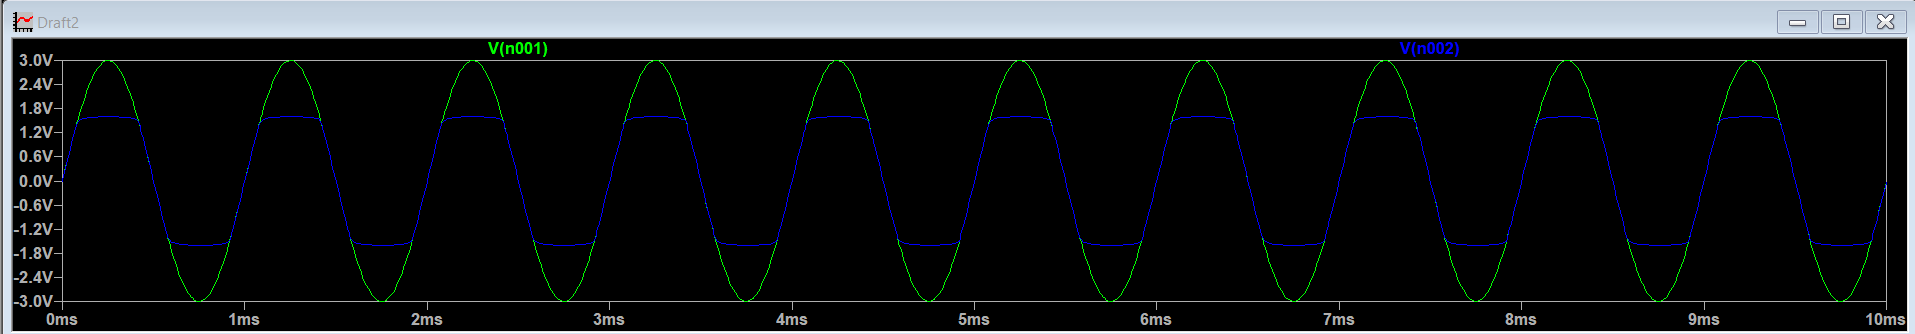
\includegraphics[width=0.85\textwidth]{E1/clipper/Biased/sim.png}
    \caption{Biased clipper: input and output waveforms, clipped on both sides}
\end{figure}

\subsection{Observation Table -- Clippers}
\begin{table}[H]
\centering
\begin{tabular}{lcccc}
\toprule
Circuit & $V_{in}$ (Vpp) & Reference & $V_{out}$ (measured) & Waveform \\
\midrule
Positive clipper & 4 & +1 V & & attached \\
Negative clipper & 4 & $-1$ V & & attached \\
Biased clipper & 4 & $\pm1$ V & & attached \\
\bottomrule
\end{tabular}
\end{table}

\section{Clamper Circuits}

\subsection{Theory}
A clamper (DC restorer) shifts a waveform up or down by a fixed amount without changing its shape. It uses a series capacitor and a diode -- the capacitor charges up to nearly the peak input voltage during the half cycle when the diode conducts, and this charge then adds a DC offset to the signal for the rest of the cycle.

\begin{itemize}
    \item \textbf{Positive clamper}: shifts the waveform upward, fixing the minimum near a chosen level.
    \item \textbf{Negative clamper}: shifts the waveform downward, fixing the maximum near a chosen level.
\end{itemize}

The theoretical DC shift is approximately equal to the peak input amplitude minus the diode drop:
\begin{equation}
    \Delta V \approx V_{peak} - V_\gamma
\end{equation}

\subsection{Positive Clamper}
\begin{figure}[H]
    \centering
    \includegraphics[width=0.55\textwidth]{{E1/clamper/Positive clamper/ckt}.png}
    \caption{Positive clamper circuit -- LTSpice}
\end{figure}

\begin{figure}[H]
    \centering
    \includegraphics[width=0.85\textwidth]{{E1/clamper/Positive clamper/sim}.png}
    \caption{Positive clamper: input and output waveforms, DC level shifted up}
\end{figure}

\subsection{Negative Clamper}
\begin{figure}[H]
    \centering
    \includegraphics[width=0.55\textwidth]{{E1/clamper/Negative clamper/ckt}.png}
    \caption{Negative clamper circuit -- LTSpice}
\end{figure}

\begin{figure}[H]
    \centering
    \includegraphics[width=0.85\textwidth]{{E1/clamper/Negative clamper/sim}.png}
    \caption{Negative clamper: input and output waveforms, DC level shifted down}
\end{figure}

\subsection{Observation Table -- Clampers}
\begin{table}[H]
\centering
\begin{tabular}{lccc}
\toprule
Circuit & $V_{in}$ (Vpp) & Expected shift & Measured shift \\
\midrule
Positive clamper & 4 & $\approx V_{peak}-V_\gamma$ & \\
Negative clamper & 4 & $\approx V_{peak}-V_\gamma$ & \\
\bottomrule
\end{tabular}
\end{table}

\section{Calculations / Analysis}
\begin{itemize}
    \item From the PN diode forward data, the cut-in voltage $V_\gamma$ will be read off, and static resistance ($V/I$) and dynamic resistance ($\Delta V/\Delta I$) will be computed near the operating point.
    \item From the reverse data, the reverse saturation current and breakdown voltage (if seen) will be noted.
    \item From the Zener data, $V_Z$ and $R_Z = \Delta V_Z/\Delta I_Z$ will be computed from the breakdown region.
    \item For each clipper, the measured clipping level will be compared with the predicted value $V_{ref} \pm V_\gamma$.
    \item For each clamper, the measured DC shift will be compared with the theoretical value $\approx V_{peak} - V_\gamma$.
\end{itemize}

\section{Results and Conclusion}
The forward V--I characteristic of the PN junction diode was simulated in LTSpice and shows the expected exponential rise in current after the cut-in voltage. The clipper circuits (positive, negative, and biased) correctly clipped the input waveform at the set reference levels, as seen in the simulated input-output plots. The clamper circuits shifted the DC level of the waveform up or down as expected, without changing its shape. The Zener diode characteristics and the reverse-bias PN junction characteristics will be measured directly in the lab and added to the observation tables above, since these depend on the physical device behaviour rather than the simplified LTSpice diode model.

\end{document}